\chapter{Results}

mention system specs and how long it took in order to precompute

the elapse does not look that regular under the electron scanning microscope. This is why it is much less iridescent than the other specie.

In addition, the micro-geometry is highly similar among snake species, it is the geometry of the nanostructures that are highly different among species and that cause the snake to be or not be iridescent. So, even Xenopeltis would not give you very different geometry than Elaphe.

Xeno has a brownish body with no pattern that makes the iridescence more spectacular than on Ellaphe


\section{BRDF maps}
In this chapter we examine the rendered output resulting by the implementation of our BRDF models applied on different input patches such as Blaze grating or Elaphe $\ref{fig:elpahespecies}$ and Xenopeltis $\ref{fig:xenospeicies}$ snake nano-scaled surface sheds. We going to discuss and compare both, their BRDF maps $\ref{fig:brdfmapexplanation}$ and the corresponding renderings on a snake geometry $\ref{sec:snakegeomrenderings}$ for various input parameters. Last we also show a real experimental image showing the effect of diffraction for similar parameters like we have. 
A BRDF map shows a shader's output for all possible viewing directions for a given, fixed, incident light direction. We assume that each viewing direction is in spherical coordinates form $\ref{sec:sphericalcoordinates}$ $(\theta_v, \phi_v)$ and is represented in the map at point $(x,y) = (sin(\theta_v)cos(\phi_v), sin(\theta_v)sin(\phi_v))$ with its origin at the map-center. The light direction for normal incidence $(\theta_i, \phi_i)$ has been fixed to $(0,\pi)$ for our rendered results.

\begin{figure}[H]
  \centering
  \subfigure[BRDF map schema]{
    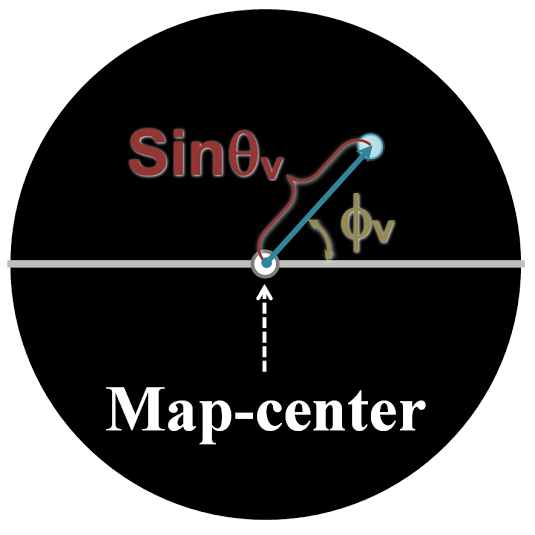
\includegraphics[scale=0.53]{results/brdfmapschema.png}
    \label{fig:brdfmapschema}
  }
~
  \subfigure[Light reflection geometrical setting]{
    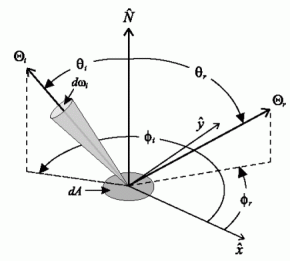
\includegraphics[scale=0.68]{results/Lightreflectiongeometry.png}
    \label{fig:lightreflectiongeometry}
  }
~

\caption{BRDF maps for different patches: $\Theta=(\theta,\phi)$ is the direction of light propagation}
\label{fig:brdfmapexplanation}
\end{figure}

In this chapter we examine the rendered output resulting by the implementation of our BRDF models applied on different input patches $\ref{fig:gratingpatches}$ such as Blaze grating or Elaphe $\ref{fig:elpahespecies}$ and Xenopeltis $\ref{fig:xenospeicies}$ snake nano-scaled surface sheds. We going to discuss and compare both, their BRDF maps $\ref{fig:brdfmapexplanation}$ and the corresponding renderings on a snake geometry $\ref{sec:snakegeomrenderings}$ for various input parameters. Last we also show a real experimental image showing the effect of diffraction for similar parameters like we have. 
A BRDF map shows a shader's output for all possible viewing directions for a given, fixed, incident light direction. We assume that each viewing direction is in spherical coordinates form $\ref{sec:sphericalcoordinates}$ $(\theta_v, \phi_v)$ and is represented in the map at point $(x,y) = (sin(\theta_v)cos(\phi_v), sin(\theta_v)sin(\phi_v))$ with its origin at the map-center. The light direction for normal incidence $(\theta_i, \phi_i)$ has been fixed to $(0,\pi)$ for our rendered results.

\begin{figure}[H]
  \centering
  \subfigure[Blaze grating with scale of 2.500 $\mu m$]{
    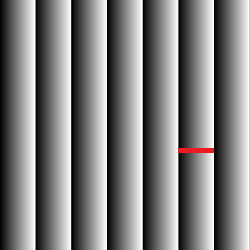
\includegraphics[scale=0.5]{evaluation/blaze_res.png}
    \label{fig:blazegratingpatch}
  }
~
  \subfigure[Elaphe patch with scale of 3.270 $\mu m$]{
    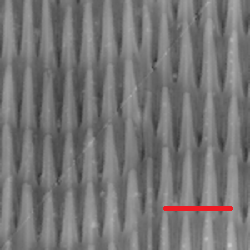
\includegraphics[scale=0.5]{evaluation/elaphe_res.png}
    \label{fig:elpahegratingpatch}
  }
~
  \subfigure[Xenopeltis patch with scale of 3.210 $\mu m$]{
    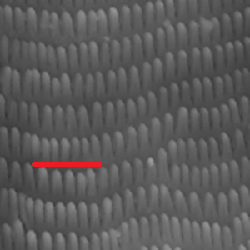
\includegraphics[scale=0.5]{evaluation/xeno_res.png}
    \label{fig:xenogratingpatch}
  }

\caption{Cutouts of our nano-scaled surface gratings used for rendering within our shader with a scale indicator (red line) for each patch. Note that for rendering we use larger patches.}
\label{fig:gratingpatches}
\end{figure}

Figure $\ref{fig:brdfmapsdiffpatches}$ shows the BRDF maps of the full lambda space sampling approach $\ref{sec:fragmentshader}$ applied on different nanoscale surface gratings as shown in figure $\ref{fig:gratingpatches}$. In Subfigure $\ref{fig:blazegratingpatch}$ we see the BRDF map for the Blazed grating, showing high relative brightness for its first order diffraction which means that for the Blazed gratings most of the diffracted spectral energy lies in its first order. Note that for Blazed grating their first-order diffracted light returns along the same path as the incident light. Higher diffraction orders are still perceivable (second and third order diffraction) but with a much lower relative brightness. The asymmetry of the pattern is due to the asymmetric geometry of the grating $\ref{fig:blazegratingpatch}$.

The finger-like structures contained in the Elaphe surface grating $\ref{fig:elpahegratingpatch}$ are quite regularly aligned and hence diffraction occurs along the horizontal axis for the BRDF map as shown in figure $\ref{fig:brdfmapElaphe}$. The reason for not seeing any strong diffraction color contribution along other directions in the BRDF map is due to the fact that these ‘nano-fingers’ overlap across layers and thus do not exhibit any definite periodicity along finger direction.

For Xenopeltis surface grating $\ref{fig:xenogratingpatch}$, we observe diffraction along many different, almost in vertical directions in the BRDF map $\ref{fig:brdfmapXeno}$ since the layers of the finger-like structures do not overlap and are shifted significantly along their length but still exhibit some local consistency. A similar argument holds true for diffraction across locally periodic finger patches with slightly different orientations. 


% brdf maps patches
\begin{figure}[H]
  \centering
  \subfigure[Blazed grating]{
    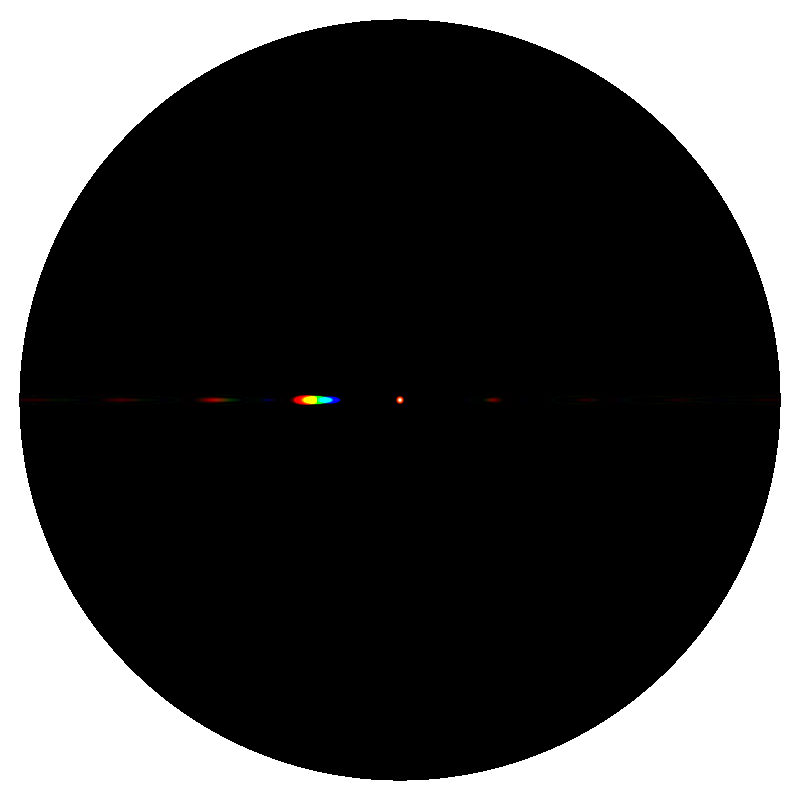
\includegraphics[scale=0.12]{results/diffPatches/fftBlazeHeight_0.25Microns_allL_weak_scale.png}
    \label{fig:brdfmapBlaze}
  }
~
  \subfigure[Elaphe grating]{
    \includegraphics[scale=0.12]{results/diffPatches/elaph65.png}
    \label{fig:brdfmapElaphe}
  }
~
  \subfigure[Xenopeltis grating]{
    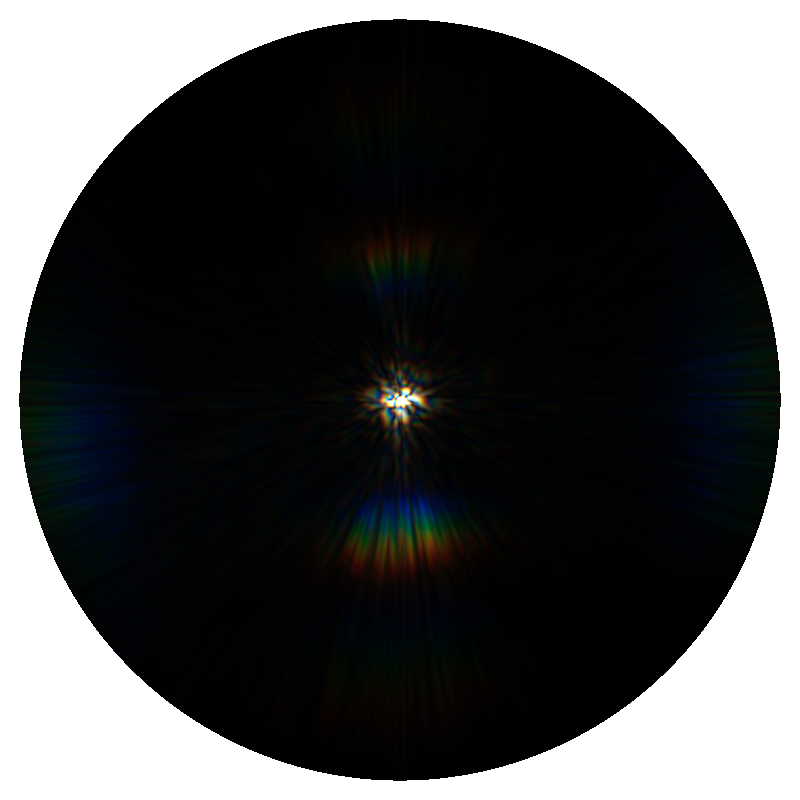
\includegraphics[scale=0.12]{results/diffPatches/xeno65.png}
    \label{fig:brdfmapXeno}
  }

\caption{BRDF maps for different patches}
\label{fig:brdfmapsdiffpatches}
\end{figure}

TODO:  CHANGE PQ, N MIN MAX IMAGE SINCE SINC INTERPOL IS MISSING
Figure $\ref{fig:brdfmapsdiffrenderingapproaches}$ shows a the BRDF maps of all our BRDF models applied on the Blaze grating. The most left figure $\ref{fig:brdfmapblazeallLambda}$ is showing the ground truth result for the Blazed grating used in order to compare with our other rendering approaches.

Figure $\ref{fig:brdfmapblazeonlyreq}$ shows the BRDF map for the $N_{min}, N_{max}$ approach which we assume to be close to the ground truth since its corresponding evaluation plots $\ref{fig:blazneval}$ already were closely matching. Nevertheless there is a small difference notable: since in the actual technical implementation of the $N_{min}, N_{max}$ shading approach treats the center of the BRDF map as a separate case, i.e. everything around a small $\epsilon$-circumference has white color assigned 
we note a white circular spot around the map center. Except this fact, the BRDF map resembles the ground truth.

Figure $\ref{fig:brdfmapblazepq}$ shows the BRDF map for the PQ approach which relies on sinc-interpolation. As expected, after having considered the corresponding evaluation plots shown in figure$\ref{fig:blazepqeval}$, the PQ BRDF map and the ground truth are visual alike. Compared to the evaluation plots, the PQ BRDF maps even persuade more. One difference we notice is that the first order is a little spread. This effect is would be strengthened when using linear interpolation instead of sinc-interpolation.

Last, let us consider figure $\ref{fig:brdfmapblazegem}$ which shows the BRDF map produced by using the implementation of Nvidia Gem's implementation (ADD REFERENCE) of Stam's BRDF model, when constrainting the y-axisis of the BRDF map. This model does not consider much more than the spacing $d$ of a given grating. It also always produces highly symmetric results. It also does not render different orders of diffraction rather than the zero and first order.   

% brdf maps patches
\begin{figure}[H]
  \centering
  \subfigure[ALL lambda]{
    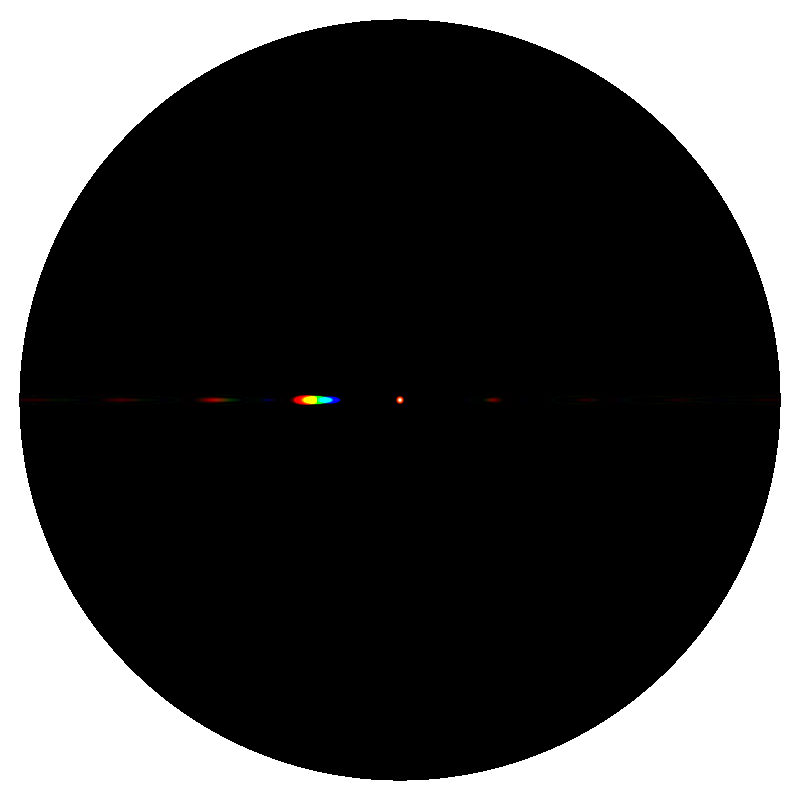
\includegraphics[scale=0.09]{results/diffPatches/fftBlazeHeight_0.25Microns_allL_weak_scale.png}
    \label{fig:brdfmapblazeallLambda}
  }
~
  \subfigure[Nmin Nmax]{
    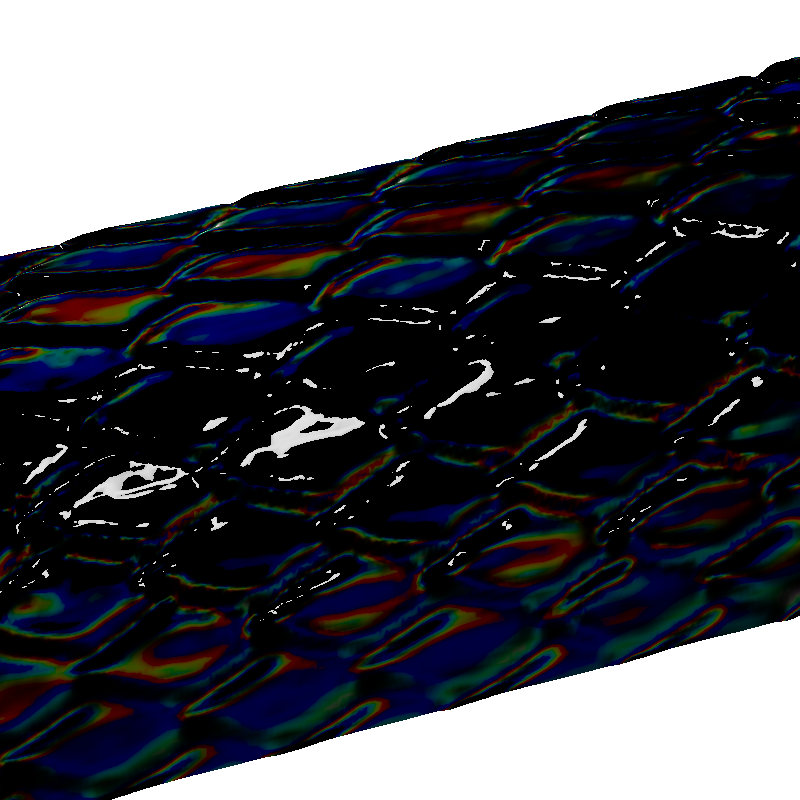
\includegraphics[scale=0.09]{results/methodComp/gem.png}
    \label{fig:brdfmapblazeonlyreq}
  }
~
  \subfigure[PQ]{
    \includegraphics[scale=0.09]{results/PQapproach_vs_sampleAll/blaze/pq.png}
    \label{fig:brdfmapblazepq}
  }
~
  \subfigure[Gem]{
    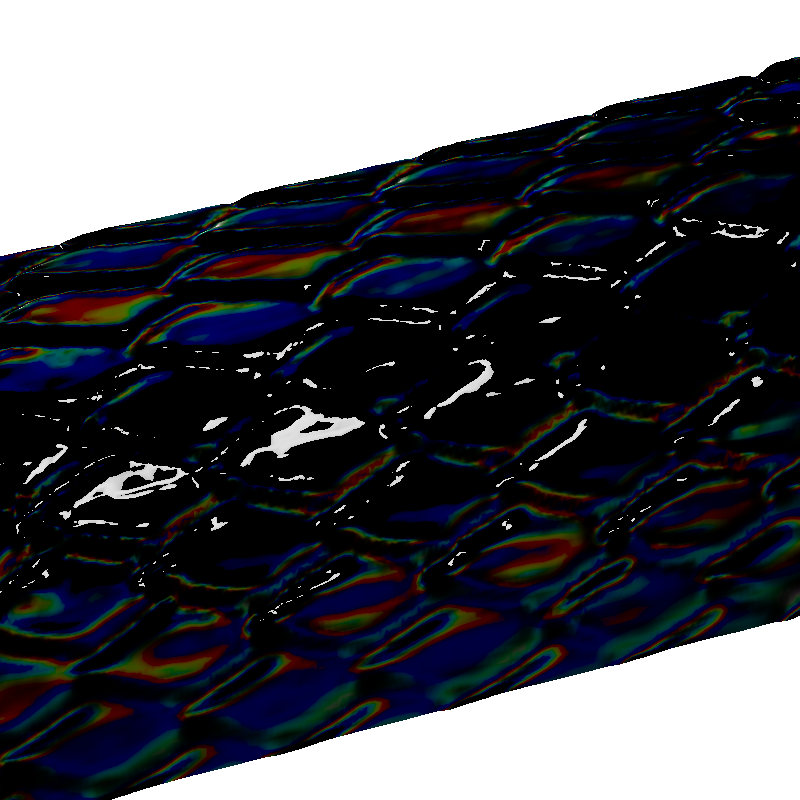
\includegraphics[scale=0.09]{results/methodComp/gem.png}
    \label{fig:brdfmapblazegem}
  }
    
\caption{BRDF maps for Blaze grating comparing our different rendering apporaches}
\label{fig:brdfmapsdiffrenderingapproaches}
\end{figure}

Figure $\ref{fig:brdfmapsdifflambdastepsblaze}$ and figure $\ref{fig:brdfmapsdifflambdastepselaphe65}$ show the BRDF maps for different wavelength step sizes used in the fragment shader for the full lambda space sampling approach applied on the Blaze grating and the Elpahe snake shed, respectively. Within our fragment shaders the most outer loop iterate over the range $[380nm, 700nm]$ for fixed step sizes $\lambda_{step}$ which basically constitutes the integration over the wavelength spectrum. Therefore, having bigger step sizes implies having fewer step sizes which will fasten up the overall runtime of a shader but will also introduce artifacts and therefore lower the overall shading qualtity. For Elaphe surface grating, artifacts are perceptional arising when $\lambda_{step} \leq 10nm$. Results produced by using $5nm$ step sizes do not differ from those produced by using $\lambda_{step}= 1nm$ which allows us to set $\lambda_{step}$ equal 5nm. For a Blazed grating we may chose even bigger step sized without losing any rendering quality.   

% blaze steps
\begin{figure}[H]
  \centering
  \subfigure[$\lambda_{step=1 nm}$]{
    \includegraphics[scale=0.12]{results/different_lambda_steps/blaze/dl=1.png}
    \label{fig:brdfmapsDiffLambdaStepsL1Blaze}
  }
~
  \subfigure[$\lambda_{step=5 nm}$]{
    \includegraphics[scale=0.12]{results/different_lambda_steps/blaze/dl=5.png}
    \label{fig:brdfmapsDiffLambdaStepsL5Blaze}
  }
~
  \subfigure[$\lambda_{step=10 nm}$]{
    \includegraphics[scale=0.12]{results/different_lambda_steps/blaze/dl=10.png}
    \label{fig:brdfmapsDiffLambdaStepsL10Blaze}
  }
  
  \subfigure[$\lambda_{step=25 nm}$]{
    \includegraphics[scale=0.12]{results/different_lambda_steps/blaze/dl=25.png}
    \label{fig:brdfmapsDiffLambdaStepsL25Blaze}
  }
~
  \subfigure[$\lambda_{step=50 nm}$]{
    \includegraphics[scale=0.12]{results/different_lambda_steps/blaze/dl=50.png}
    \label{fig:brdfmapsDiffLambdaStepsL50Blaze}
  }
~ 
  \subfigure[$\lambda_{step=100 nm}$]{
    \includegraphics[scale=0.12]{results/different_lambda_steps/blaze/dl=100.png}
    \label{fig:brdfmapsDiffLambdaStepsL100Blaze}
  }
  
\caption{Blaze grating at $2.5 \mu m$: Different $\lambda$ step sizes}
\label{fig:brdfmapsdifflambdastepsblaze}
\end{figure}

% elpahe steps
\begin{figure}[H]
  \centering
  \subfigure[$\lambda_{step=1 nm}$]{
    \includegraphics[scale=0.12]{results/different_lambda_steps/elaphe65/dl=1.png}
    \label{fig:brdfmapsDiffLambdaStepsL1Elaphe65}
  }
~
  \subfigure[$\lambda_{step=5 nm}$]{
    \includegraphics[scale=0.12]{results/different_lambda_steps/elaphe65/dl=5.png}
    \label{fig:brdfmapsDiffLambdaStepsL5Elaphe65}
  }
~
  \subfigure[$\lambda_{step=10 nm}$]{
    \includegraphics[scale=0.12]{results/different_lambda_steps/elaphe65/dl=10.png}
    \label{fig:brdfmapsDiffLambdaStepsL10Elaphe65}
  }
  
  \subfigure[$\lambda_{step=25 nm}$]{
    \includegraphics[scale=0.12]{results/different_lambda_steps/elaphe65/dl=25.png}
    \label{fig:brdfmapsDiffLambdaStepsL25Elaphe65}
  }
~
  \subfigure[$\lambda_{step=50 nm}$]{
    \includegraphics[scale=0.12]{results/different_lambda_steps/elaphe65/dl=50.png}
    \label{fig:brdfmapsDiffLambdaStepsL50Elaphe65}
  }
~ 
  \subfigure[$\lambda_{step=100 nm}$]{
    \includegraphics[scale=0.12]{results/different_lambda_steps/elaphe65/dl=100.png}
    \label{fig:brdfmapsDiffLambdaStepsL100Elaphe65}
  }
  
\caption{Elaphe grating at $65 \mu m$: Different $\lambda$ step sizes}
\label{fig:brdfmapsdifflambdastepselaphe65}
\end{figure}


The Figures $\ref{fig:pqblaze}$, $\ref{fig:pqxeno}$, $\ref{fig:pqelaphe}$ show a comparison of the BRDF maps produced by full lambda space sampling approach (on the left) and the PQ shading approach (on the right) applied on all our patches. For Blazed grating, as already mentioned, we notice that both approaches resemble each other. We also notice that for PQ map, the first order diffraction color contribution is spread. For Elaphe and Xenopeltis grating we notice similar shaped BRDF patterns, even when the angle of light varies, but nevertheless, they also contain some artifacts. This also holds true for 

%pq blaze
\begin{figure}[H]
  \centering
  \subfigure[Full Lambda Sampling: Blaze grating]{
    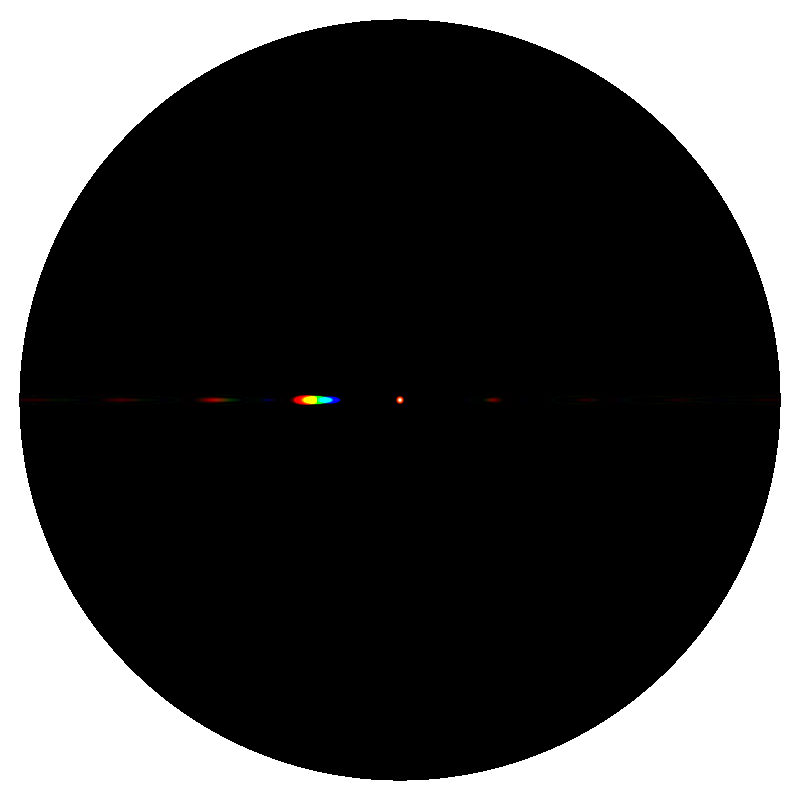
\includegraphics[scale=0.12]{results/PQapproach_vs_sampleAll/blaze/fftBlazeHeight_0.25Microns_allL_weak_scale_g=1.1.png}
    \label{fig:fullLambdaBlaze}
  }
~
  \subfigure[Full Lambda Sampling brightened: Blaze grating]{
            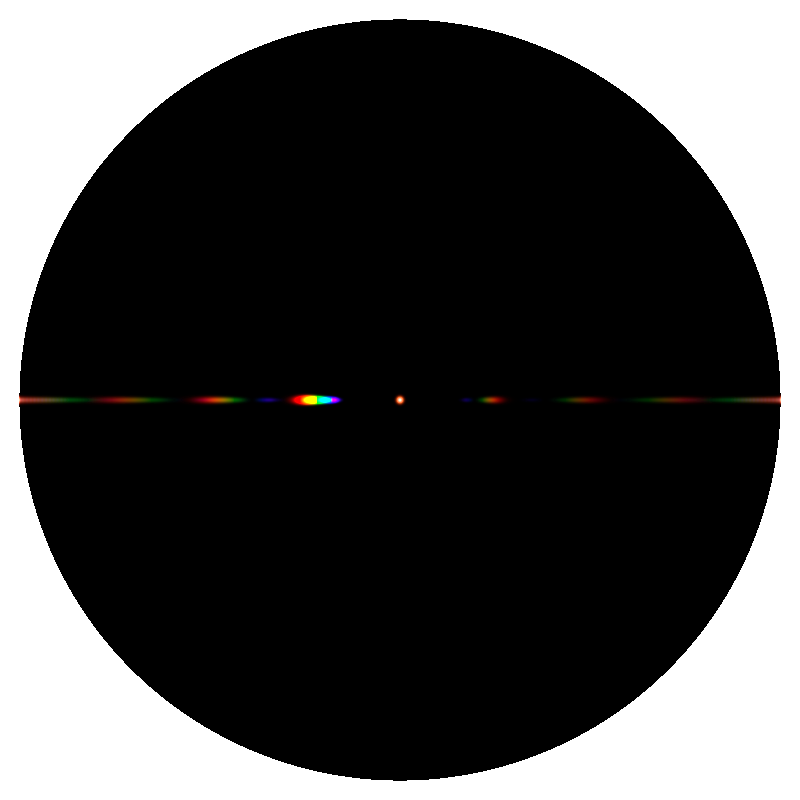
\includegraphics[scale=0.12]{results/PQapproach_vs_sampleAll/blaze/fftBlazeHeight_0.25Microns_allL_weak_scale_g=2.2_scale=100.png}
    \label{fig:fullLambdaBrightenedBlaze}
  }
~
  \subfigure[PQ Approach: Blaze grating]{
    \includegraphics[scale=0.12]{results/PQapproach_vs_sampleAll/blaze/pq.png}
    \label{fig:pqBlaze}
  }
  
\caption{Blaze grating: PQ approach vs full lambda space sampling}
\label{fig:pqblaze}
\end{figure}

%pq elaphe
\begin{figure}[H]
  \centering
  \subfigure[Full Lambda Sampling: Elaphe grating]{
    \includegraphics[scale=0.2]{results/PQapproach_vs_sampleAll/elaphe/elaph65.png}
    \label{fig:fullLambdaElaphe}
  }
~
  \subfigure[PQ Approach: Elaphe grating]{
    \includegraphics[scale=0.2]{results/PQapproach_vs_sampleAll/elaphe/pq.png}
    \label{fig:pqElaphe}
  }

  
\caption{Elaphe grating: PQ approach vs full lambda space sampling}
\label{fig:pqelaphe}
\end{figure}

%pq xeno
\begin{figure}[H]
  \centering
  \subfigure[Full Lambda Sampling: Xeno grating $\theta_i = 0 degree$]{
    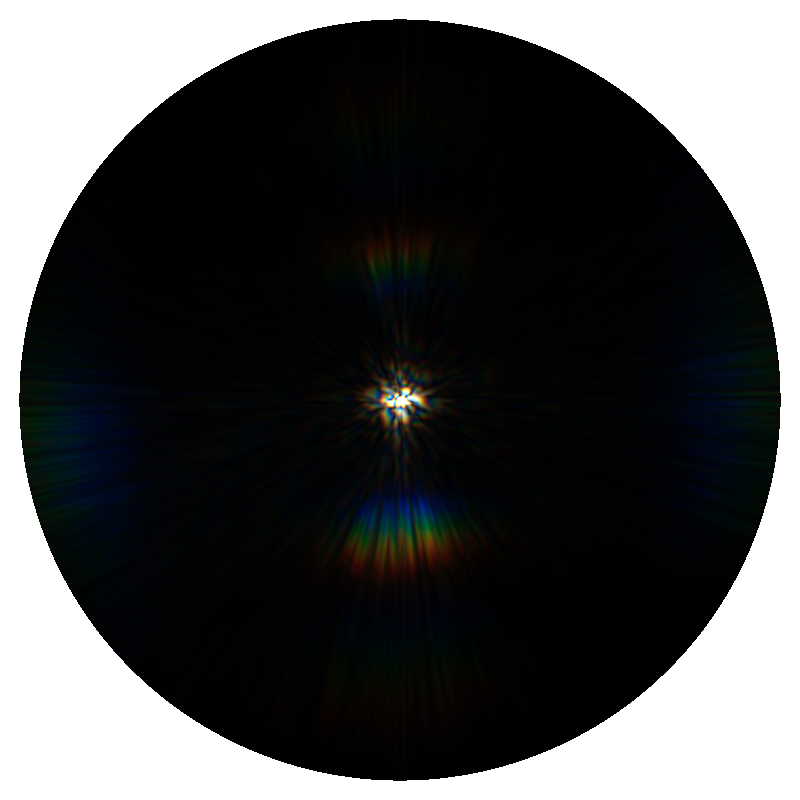
\includegraphics[scale=0.19]{results/PQapproach_vs_sampleAll/xeno/a_xeno_t_i=0.png}
    \label{fig:fullLambdaXenoti0}
  }
~
  \subfigure[PQ Approach: Xeno grating $\theta_i = 0 degree$]{
    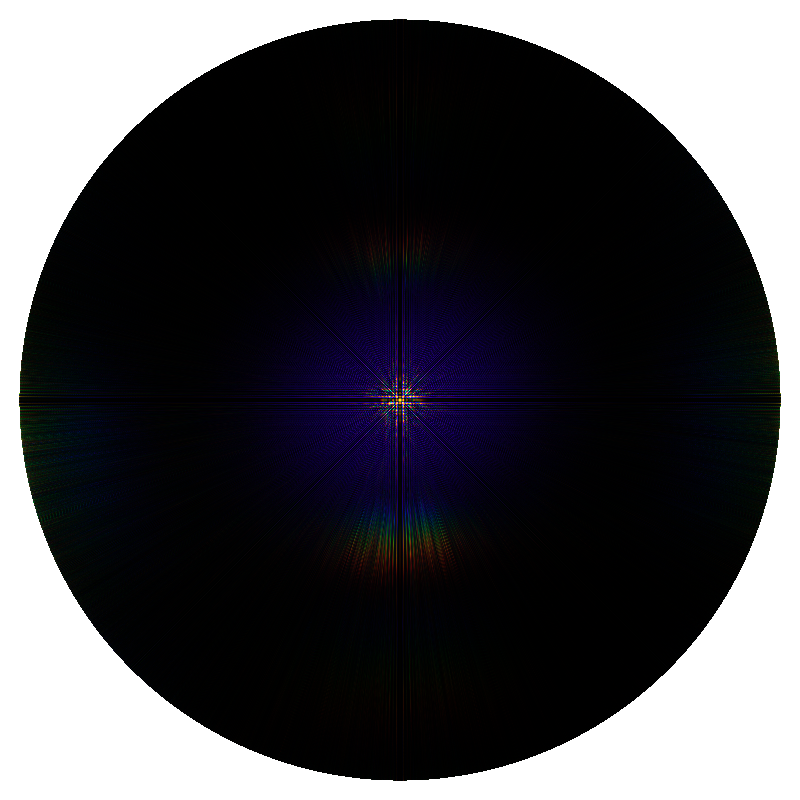
\includegraphics[scale=0.19]{results/PQapproach_vs_sampleAll/xeno/a_pq_t_i=0.png}
    \label{fig:pqXenoti0}
  }

  \subfigure[Full Lambda Sampling: Xeno grating $\theta_i = 10 degree$]{
    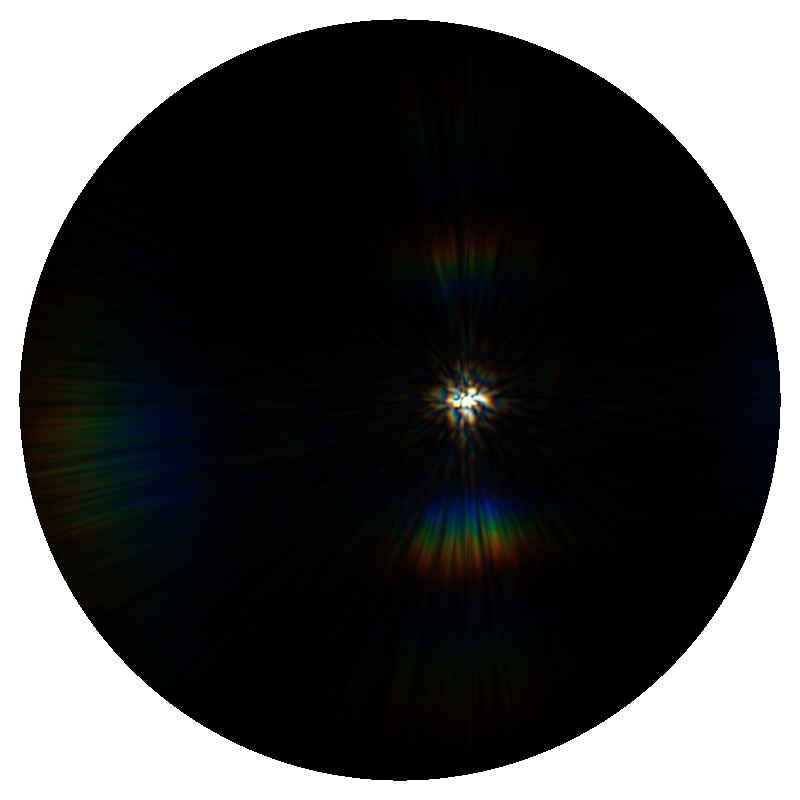
\includegraphics[scale=0.19]{results/PQapproach_vs_sampleAll/xeno/b_xeno_t_i=10.png}
    \label{fig:fullLambdaXenoti10}
  }
~
  \subfigure[PQ Approach: Xeno grating $\theta_i = 10 degree$]{
    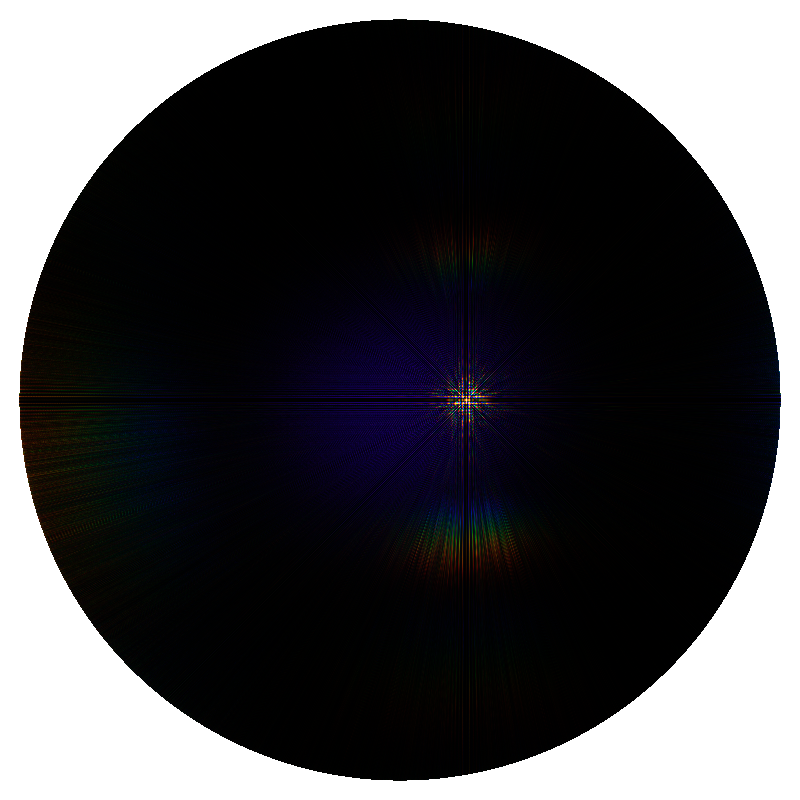
\includegraphics[scale=0.19]{results/PQapproach_vs_sampleAll/xeno/b_pq_t_i=10.png}
    \label{fig:pqXenoti10}
  }
  
  \subfigure[Full Lambda Sampling: Xeno grating $\theta_i = 20 degree$]{
    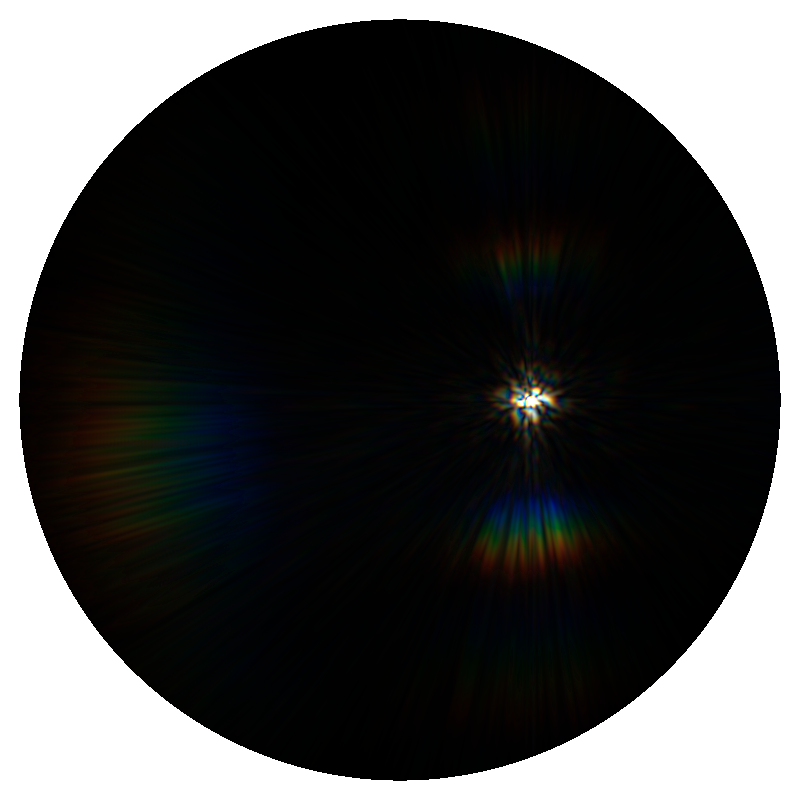
\includegraphics[scale=0.19]{results/PQapproach_vs_sampleAll/xeno/c_xeno_t_i=20.png}
    \label{fig:fullLambdaXenoti20}
  }
~
  \subfigure[PQ Approach: Xeno grating $\theta_i = 20 degree$]{
    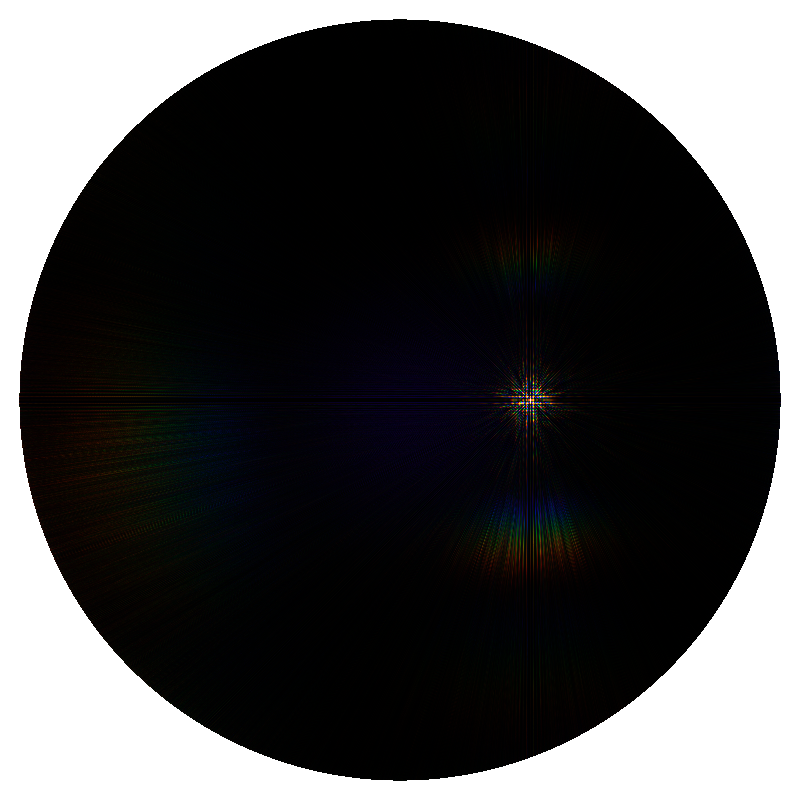
\includegraphics[scale=0.19]{results/PQapproach_vs_sampleAll/xeno/c_pq_t_i=20.png}
    \label{fig:pqXenoti20}
  }
  
\caption{Xeno grating: PQ approach vs full lambda space sampling}
\label{fig:pqxeno}
\end{figure}

Figure $\ref{fig:brdfmapsdiffsigmasizeblaze}$ shows BRDF map for full lambda sampling approach applied on the Blaze grating, varying the value for the spacial variance $\sigma_s$.
blaze grating lower coherence length, fewer interacting grating periods, produce blurred diffraction bands for different lambda which overlap to produce poorly resolved colors.

%sigma var
\begin{figure}[H]
  \centering
  \subfigure[$\sigma_{s=3.25 \mu m}$]{
    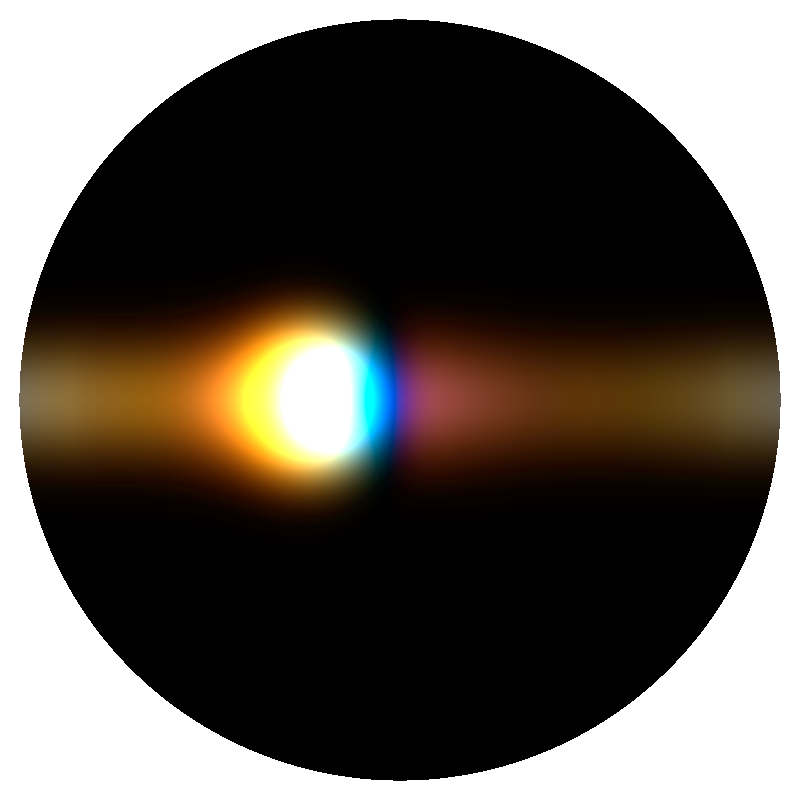
\includegraphics[scale=0.12]{results/sigma_sVariation/blaze/sigma_s=3.25.png}
    \label{fig:brdfmapsDiffSigmaStepsL1Blaze}
  }
~
  \subfigure[$\sigma_{s=6.5 \mu m}$]{
    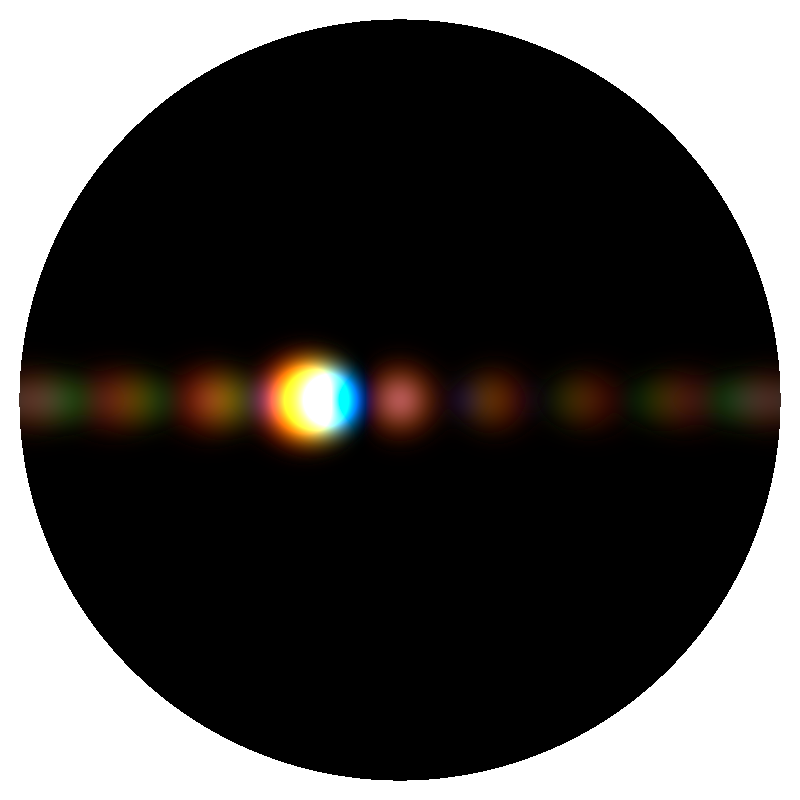
\includegraphics[scale=0.12]{results/sigma_sVariation/blaze/sigma_s=6.5.png}
    \label{fig:brdfmapsDiffSigmaStepsL5Blaze}
  }
~
  \subfigure[$\sigma_{s=15 \mu m}$]{
    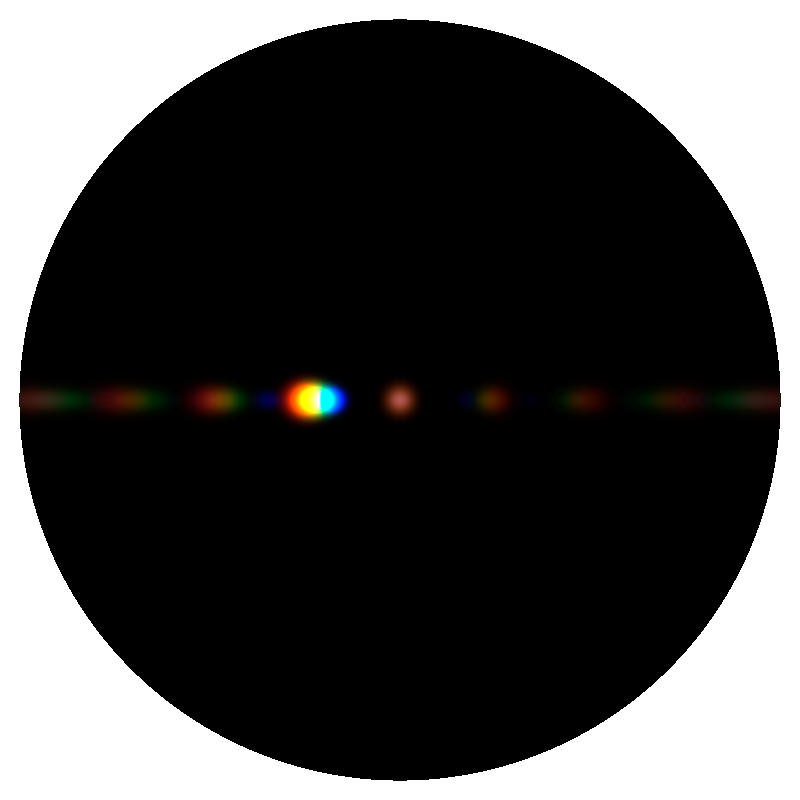
\includegraphics[scale=0.12]{results/sigma_sVariation/blaze/sigma_s=15.png}
    \label{fig:brdfmapsDiffSigmaStepsL10Blaze}
  }
  
  \subfigure[$\sigma_{s=30 \mu m}$]{
    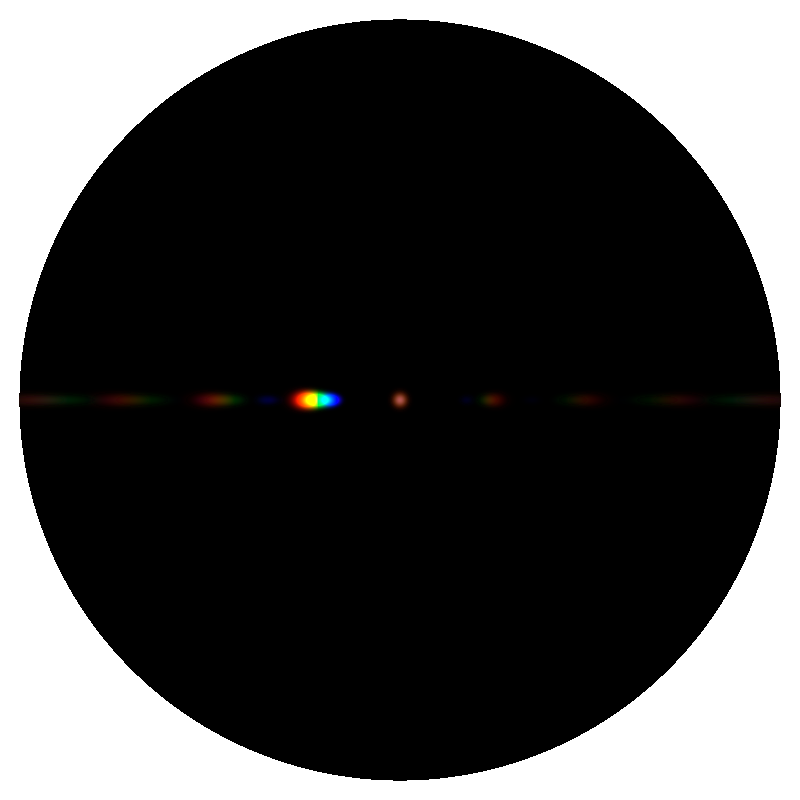
\includegraphics[scale=0.12]{results/sigma_sVariation/blaze/sigma_s=30.png}
    \label{fig:brdfmapsDiffSigmaStepsL25Blaze}
  }
~
  \subfigure[$\sigma_{s=45 \mu m}$]{
    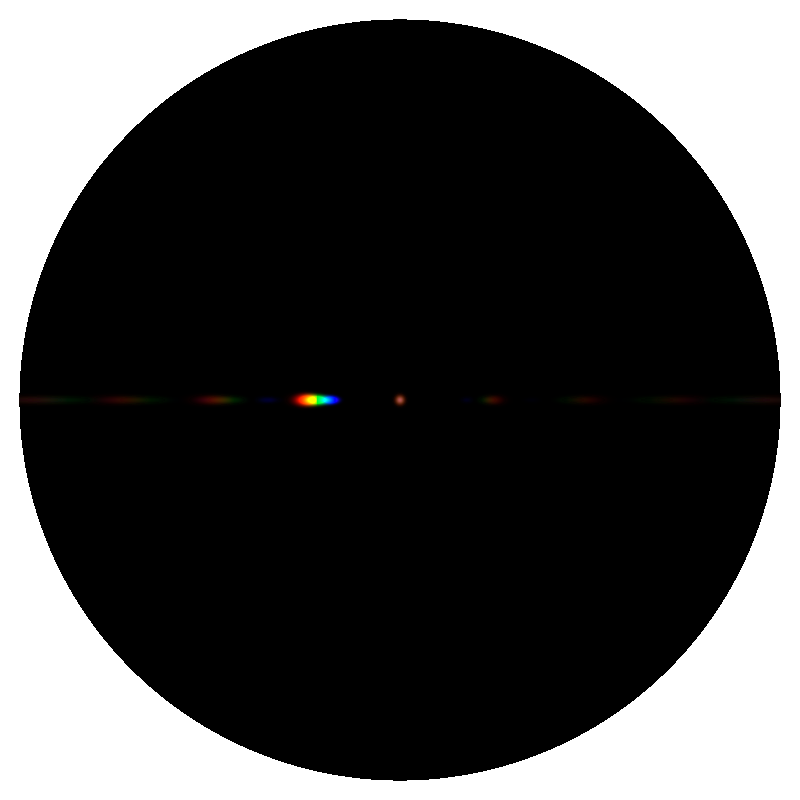
\includegraphics[scale=0.12]{results/sigma_sVariation/blaze/sigma_s=45.png}
    \label{fig:brdfmapsDiffSigmaStepsL50Blaze}
  }
~ 
  \subfigure[$\sigma_{s=65 \mu m}$]{
    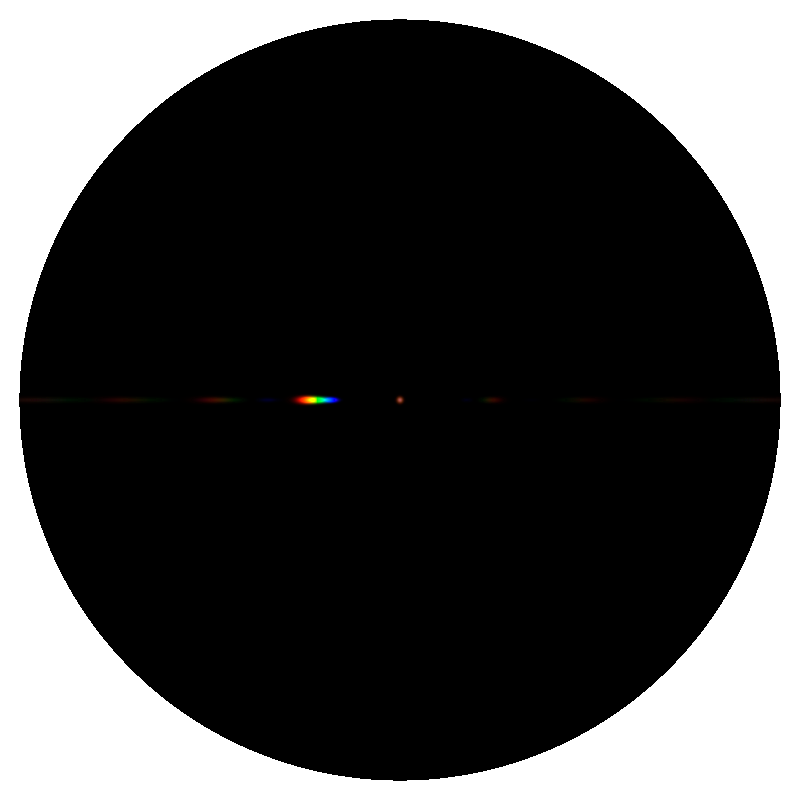
\includegraphics[scale=0.12]{results/sigma_sVariation/blaze/sigma_s=65.png}
    \label{fig:brdfmapsDiffSigmaStepsL100Blaze}
  }
  
  
\caption{Blaze grating at $2.5 \mu m$: Different $\sigma_s$ sizes}
\label{fig:brdfmapsdiffsigmasizeblaze}
\end{figure}

The figures $\ref{fig:brdfmapstayloriterationsblaze}$ and $\ref{fig:brdfmapstayloriterationselaphe65}$ show the BRDF maps of the full lambda space approach using different values for $N$ used for the taylor series approximation used within our fragment shaders. For both input patches we clearly visually observe the convergence of the taylor series for higher values for N.

%taylor var blaze
\begin{figure}[H]
  \centering
  \subfigure[$N=0$]{
    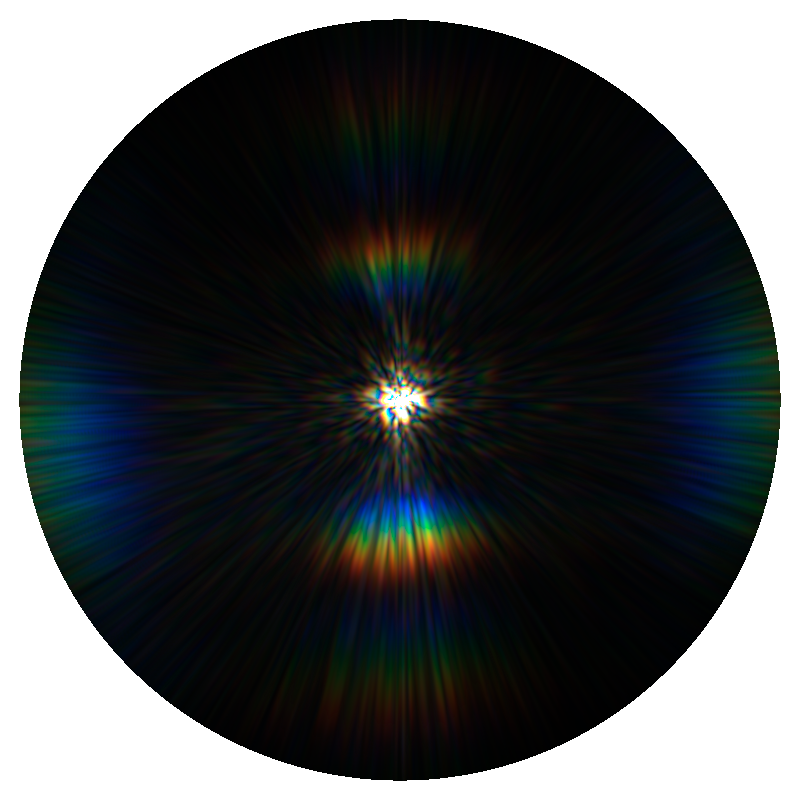
\includegraphics[scale=0.06]{results/taylorStepsVar/blaze/0.png}
    \label{fig:brdfmapsTaylorN0Blaze}
  }
~
  \subfigure[$N=1$]{
    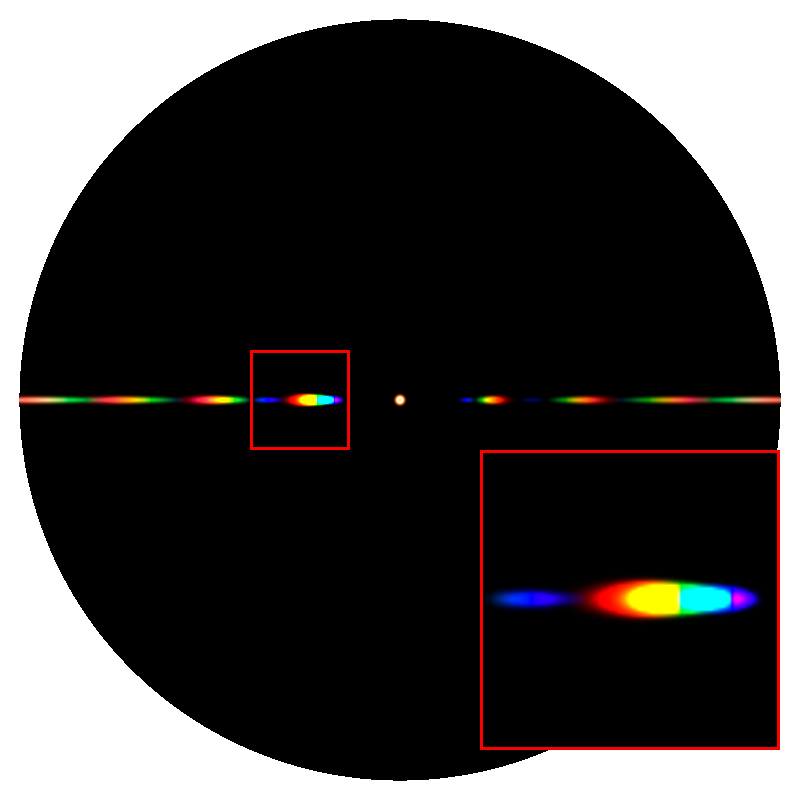
\includegraphics[scale=0.06]{results/taylorStepsVar/blaze/1.png}
    \label{fig:brdfmapsTaylorN1Blaze}
  }
~
  \subfigure[$N=2$]{
    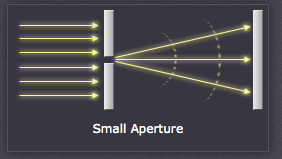
\includegraphics[scale=0.06]{results/taylorStepsVar/blaze/2.png}
    \label{fig:brdfmapsTaylorN2Blaze}
  }
~  
  \subfigure[$N=3$]{
    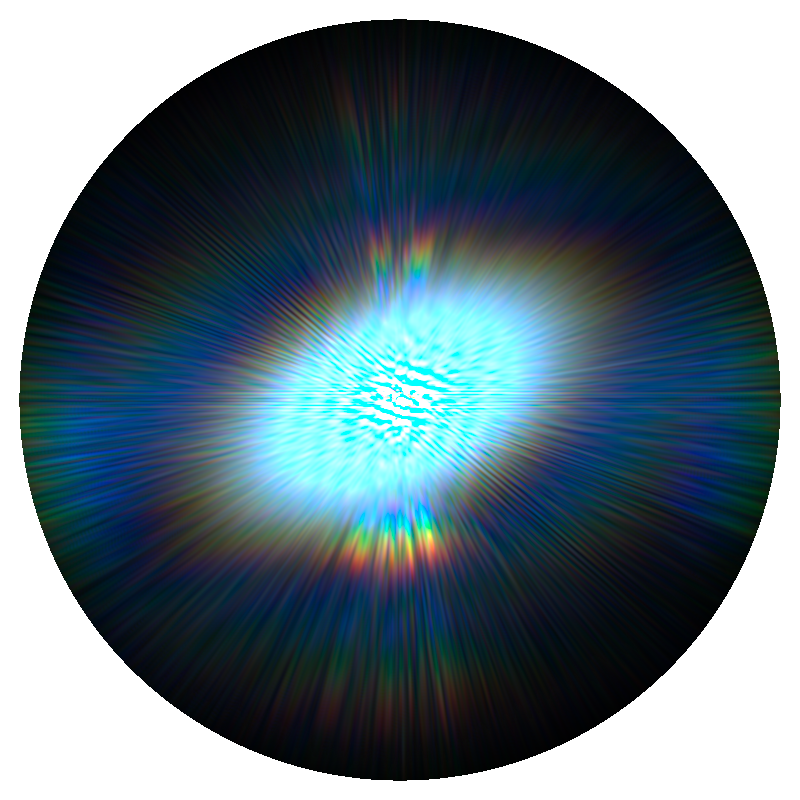
\includegraphics[scale=0.06]{results/taylorStepsVar/blaze/3.png}
    \label{fig:brdfmapsTaylorN3Blaze}
  }
~
  \subfigure[$N=4$]{
    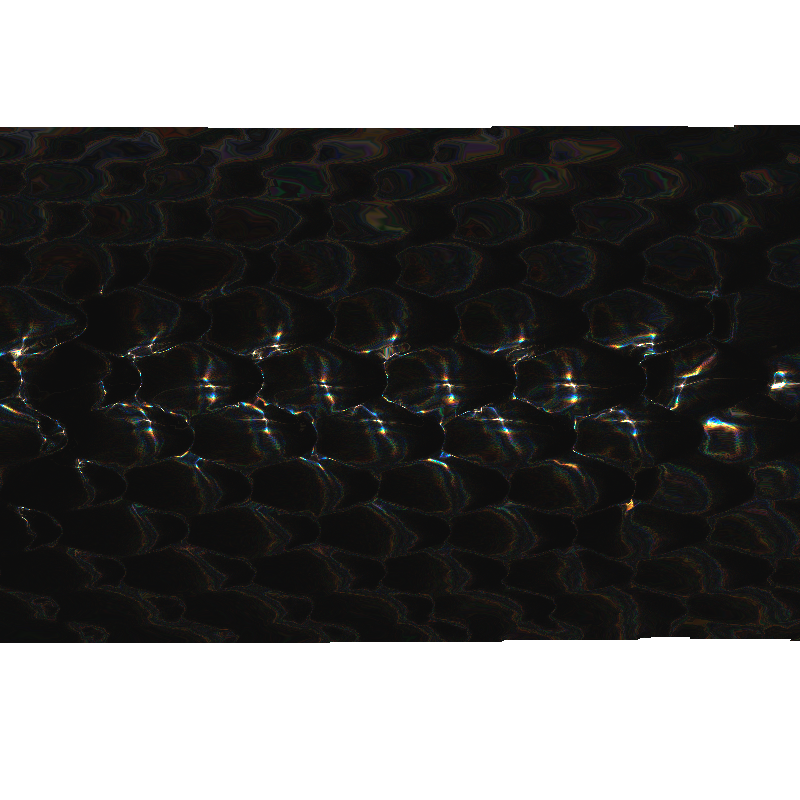
\includegraphics[scale=0.06]{results/taylorStepsVar/blaze/4.png}
    \label{fig:brdfmapsTaylorN4Blaze}
  }

  \subfigure[$N=5$]{
    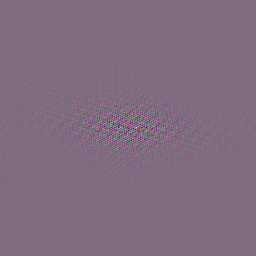
\includegraphics[scale=0.06]{results/taylorStepsVar/blaze/5.png}
    \label{fig:brdfmapsTaylorN5Blaze}
  }
~  
  \subfigure[$N=6$]{
    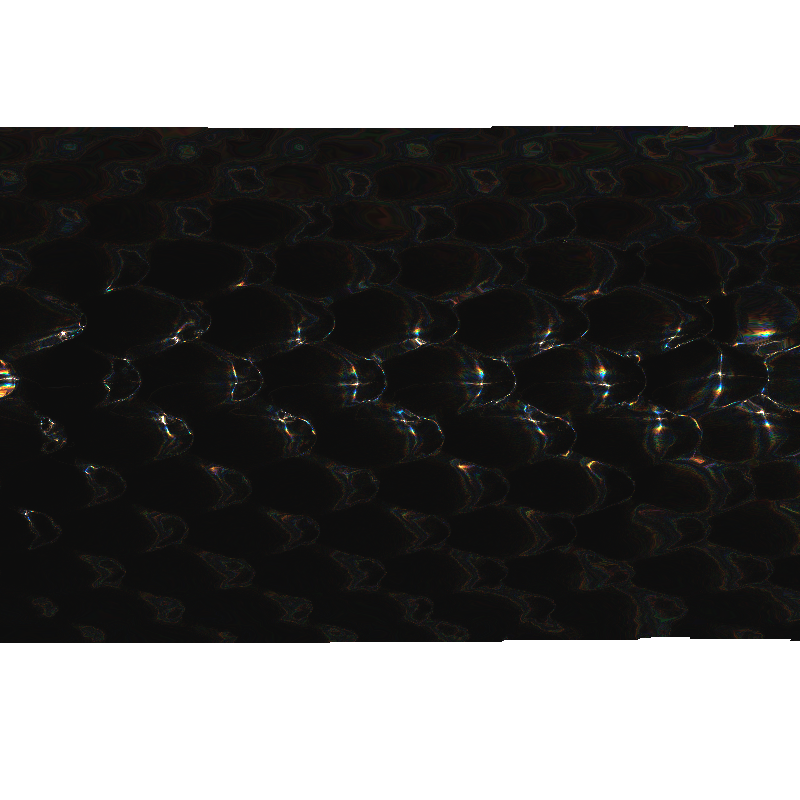
\includegraphics[scale=0.06]{results/taylorStepsVar/blaze/6.png}
    \label{fig:brdfmapsTaylorN6Blaze}
  }
~  
  \subfigure[$N=7$]{
    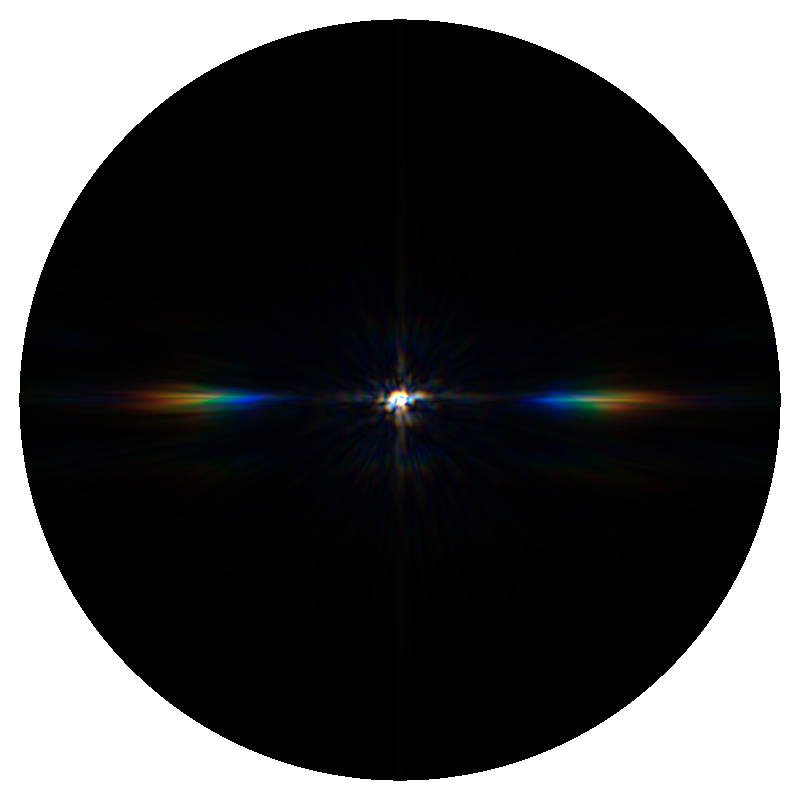
\includegraphics[scale=0.06]{results/taylorStepsVar/blaze/7.png}
    \label{fig:brdfmapsTaylorN7Blaze}
  }
~  
  \subfigure[$N=8$]{
    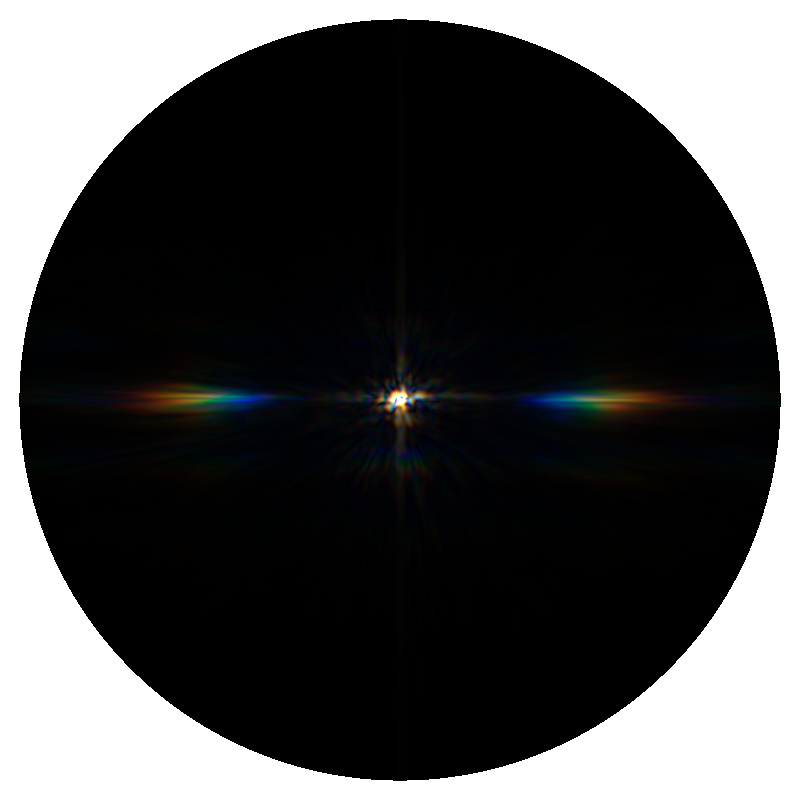
\includegraphics[scale=0.06]{results/taylorStepsVar/blaze/8.png}
    \label{fig:brdfmapsTaylorN8Blaze}
  }
~ 
  \subfigure[$N=9$]{
    \includegraphics[scale=0.06]{results/taylorStepsVar/blaze/9.png}
    \label{fig:brdfmapsTaylorN9Blaze}
  }
  
  
\caption{Blaze grating at $2.5 \mu m$: $N$ Taylor Iterations}
\label{fig:brdfmapstayloriterationsblaze}
\end{figure}

%taylor var elaphe
\begin{figure}[H]
  \centering
  \subfigure[$N=0$]{
    \includegraphics[scale=0.06]{results/taylorStepsVar/elaphe65/0.png}
    \label{fig:brdfmapsTaylorN0Elaphe65}
  }
~
  \subfigure[$N=1$]{
    \includegraphics[scale=0.06]{results/taylorStepsVar/elaphe65/1.png}
    \label{fig:brdfmapsTaylorN1Elaphe65}
  }
~
  \subfigure[$N=2$]{
    \includegraphics[scale=0.06]{results/taylorStepsVar/elaphe65/2.png}
    \label{fig:brdfmapsTaylorN2Elaphe65}
  }
~  
  \subfigure[$N=3$]{
    \includegraphics[scale=0.06]{results/taylorStepsVar/elaphe65/3.png}
    \label{fig:brdfmapsTaylorN3Elaphe65}
  }
~
  \subfigure[$N=4$]{
    \includegraphics[scale=0.06]{results/taylorStepsVar/elaphe65/4.png}
    \label{fig:brdfmapsTaylorN4Elaphe65}
  }

  \subfigure[$N=5$]{
    \includegraphics[scale=0.06]{results/taylorStepsVar/elaphe65/5.png}
    \label{fig:brdfmapsTaylorN5Elaphe65}
  }
~  
  \subfigure[$N=6$]{
    \includegraphics[scale=0.06]{results/taylorStepsVar/elaphe65/6.png}
    \label{fig:brdfmapsTaylorN6Elaphe65}
  }
~  
  \subfigure[$N=7$]{
    \includegraphics[scale=0.06]{results/taylorStepsVar/elaphe65/7.png}
    \label{fig:brdfmapsTaylorN7Elaphe65}
  }
~  
  \subfigure[$N=8$]{
    \includegraphics[scale=0.06]{results/taylorStepsVar/elaphe65/8.png}
    \label{fig:brdfmapsTaylorN8Elaphe65}
  }
~ 
  \subfigure[$N=9$]{
    \includegraphics[scale=0.06]{results/taylorStepsVar/elaphe65/9.png}
    \label{fig:brdfmapsTaylorN9Elaphe65}
  }
  
\caption{Elaphe grating at $65 \mu m$: $N$ Taylor Iterations}
\label{fig:brdfmapstayloriterationselaphe65}
\end{figure}


Figure $\ref{fig:brdfmapsxenodiffthetaiangles}$ shows the BRDF maps of the full lambda shading approach applied on the Xenopeltis snake shed, using different $\theta_i$ incident angles.

% brdf maps xeno angles
\begin{figure}[H]
  \centering
  \subfigure[Xeno grating $\theta_i=0$]{
    \includegraphics[scale=0.12]{results/different_theta_i_angles/xenopeltis/xeno_t_i=0.png}
    \label{fig:brdfmapXenoti0}
  }
~
  \subfigure[Xeno grating $\theta_i=10$]{
    \includegraphics[scale=0.12]{results/different_theta_i_angles/xenopeltis/xeno_t_i=10.png}
    \label{fig:brdfmapXenoti10}
  }
~
  \subfigure[Xeno grating $\theta_i=20$]{
    \includegraphics[scale=0.12]{results/different_theta_i_angles/xenopeltis/xeno_t_i=20.png}
    \label{fig:brdfmapXenoti20}
  }
  
\caption{BRDF maps for Xeno grating: different $\theta_i$ angles}
\label{fig:brdfmapsxenodiffthetaiangles}
\end{figure}


\section{Snake surface geometries}
\label{sec:snakegeomrenderings}
initially using fully lambda shader for those renderings, slow but accurate.

diffraction colors change dramatically with changes in light direction, surface normals and viewing direction, which s typical for diffraction colors observed in nature.

Mention resuolution of patches and their runtimes with used hardware - specify this hardware too.


Figure $\ref{fig:renderingdifferentsnankegratings}$ shows renderings of full lambda sampling approach applied on a snake shaped mesh for different given input patches.

\begin{figure}[H]
  \centering
  \subfigure[Blaze grating]{
    \includegraphics[scale=0.12]{results/snakerenderings/compars/blaze.png}
    \label{fig:renderingBlazeGrating}
  }
~
  \subfigure[Elaphe grating]{
    \includegraphics[scale=0.12]{results/snakerenderings/compars/elaphe65.png}
    \label{fig:renderingElapheGrating}
  }
~
  \subfigure[Xeno grating]{
    \includegraphics[scale=0.12]{results/snakerenderings/compars/xeno65.png}
    \label{fig:renderingXenoGrating}
  }
  
\caption{Diffraction of different snake skin gratings rendered on a snake geometry}
\label{fig:renderingdifferentsnankegratings}
\end{figure}


Figure $\ref{fig:renderingelaphe65}$ dsfsdf

\begin{figure}[H]
  \centering
  \subfigure[Diffraction Patten]{
    \includegraphics[scale=0.2]{results/snakerenderings/elaphe65/1.png}
    \label{fig:renderingElaphe65DP}
  }
~
  \subfigure[Diffraction + Texture]{
    \includegraphics[scale=0.2]{results/snakerenderings/elaphe65/2.png}
    \label{fig:renderingElaphe65DT}
  }

  \subfigure[Texture + Lightdir]{
    \includegraphics[scale=0.12]{results/snakerenderings/elaphe65/3.png}
    \label{fig:renderingElaphe65TL}
  }
~
  \subfigure[Nanostructure]{
    \includegraphics[scale=0.10]{results/snakerenderings/elaphe65/4.png}
    \label{fig:renderingElaphe65NS}
  }
~ 
  \subfigure[Fourier Transform]{
    \includegraphics[scale=0.52]{results/snakerenderings/elaphe65/5.png}
    \label{fig:renderingElaphe65FT}
  }
  
\caption{Diffraction for Elaphe snake skin}
\label{fig:renderingelaphe65}
\end{figure}


Figure $\ref{fig:renderingxeno65}$ dsfsdf


\begin{figure}[H]
  \centering
  \subfigure[Diffraction Patten]{
    \includegraphics[scale=0.2]{results/snakerenderings/xeno65/1.png}
    \label{fig:renderingXeno65DP}
  }
~
  \subfigure[Diffraction + Texture]{
    \includegraphics[scale=0.2]{results/snakerenderings/xeno65/2.png}
    \label{fig:renderingXeno65DT}
  }

  \subfigure[Texture + Lightdir]{
    \includegraphics[scale=0.12]{results/snakerenderings/xeno65/3.png}
    \label{fig:renderingXeno65TL}
  }
~
  \subfigure[Nanostructure]{
    \includegraphics[scale=0.075]{results/snakerenderings/xeno65/4.png}
    \label{fig:renderingXeno65NS}
  }
~ 
  \subfigure[Fourier Transform]{
    \includegraphics[scale=0.52]{results/snakerenderings/xeno65/5.png}
    \label{fig:renderingXeno65FT}
  }
  
  
  
\caption{Diffraction for Xeno snake skin}
\label{fig:renderingxeno65}
\end{figure}

Figure $\ref{fig:renderingdifferentzoomlevelselaphe}$ shows the diffraction pattern for a Elaphe snake shed for different zoom levels for fixed incident light and viewing direction using the full lambda sampling approach.

\begin{figure}[H]
  \centering
  \subfigure[$zoom = 0.1$]{
    \includegraphics[scale=0.2]{results/snakerenderings/zoomIn/elaphe65/0.1.png}
    \label{fig:renderingZoomElaphe01}
  }
~
  \subfigure[$zoom = 0.2$]{
    \includegraphics[scale=0.2]{results/snakerenderings/zoomIn/elaphe65/0.2.png}
    \label{fig:renderingZoomElaphe02}
  }
  
  \subfigure[$zoom = 0.5$]{
    \includegraphics[scale=0.2]{results/snakerenderings/zoomIn/elaphe65/0.5.png}
    \label{fig:renderingZoomElaphe05}
  }
~
  \subfigure[$zoom = 1.0$]{
    \includegraphics[scale=0.2]{results/snakerenderings/zoomIn/elaphe65/1.png}
    \label{fig:renderingZoomElaphe1}
  }
  
  \subfigure[$zoom = 1.5$]{
    \includegraphics[scale=0.2]{results/snakerenderings/zoomIn/elaphe65/1.5.png}
    \label{fig:renderingZoomElaphe15}
  }
~
  \subfigure[$zoom = 2.0$]{
    \includegraphics[scale=0.2]{results/snakerenderings/zoomIn/elaphe65/2.png}
    \label{fig:renderingZoomElaphe2}
  }
  
\caption{Diffraction on Elaphe snake skin grating: Different camera zoom levels}
\label{fig:renderingdifferentzoomlevelselaphe}
\end{figure}


Figure $\ref{fig:renderingelaphelightrotations6}$ shows how the diffraction pattern changes when slightly moving the incident light direction. same to position, different from pos

% first 3 move along x, next 3 move along y
\begin{figure}[H]
  \centering
  \subfigure[$(-3.3130, 0.0, -0.9999)$]{
    \includegraphics[scale=0.12]{results/snakerenderings/rotateLight/elaphe65/moveX/2.png}
    \label{fig:renderingElapheRotX2}
  }
~
  \subfigure[$(-0.1989, 0.0, -0.9799)$]{
    \includegraphics[scale=0.12]{results/snakerenderings/rotateLight/elaphe65/moveX/4.png}
    \label{fig:renderingElapheRotX4}
  }
~
  \subfigure[$(-0.3897, 0.0, -0.9208)$]{
    \includegraphics[scale=0.12]{results/snakerenderings/rotateLight/elaphe65/moveX/6.png}
    \label{fig:renderingElapheRotX6}
  }
  
  \subfigure[$(0.0995, 0.0993, -0.9900)$]{
    \includegraphics[scale=0.12]{results/snakerenderings/rotateLight/elaphe65/moveY/2.png}
    \label{fig:renderingElapheRotY2}
  }
~
  \subfigure[$(0.0995, 0.2940, -0.9505)$]{
    \includegraphics[scale=0.12]{results/snakerenderings/rotateLight/elaphe65/moveY/4.png}
    \label{fig:renderingElapheRotY4}
  }
~
  \subfigure[$(0.0995, 0.4770, -0.8731)$]{
    \includegraphics[scale=0.12]{results/snakerenderings/rotateLight/elaphe65/moveY/6.png}
    \label{fig:renderingElapheRotY6}
  }
  
  
\caption{Diffraction on Elaphe snake skin grating: Different light directions}
\label{fig:renderingelaphelightrotations6}
\end{figure}

Figure $\ref{fig:experimentelaphe65}$ shows a photo of an experimental setup for demonstrating the effect of diffraction using a Elpahe snake grating. The exact parameters for the experimental setup are unknown. Nevertheless this image gives us an impression of how close our model is to the reality comparing it with our simulated results since we notice similar diffraction patterns for our simulated results using an Elaphe snake shed. 

\begin{figure}[H]
  \includegraphics[scale=0.2]{results/experiment/elaphe/g2.png}
  \caption{Diffraction Elaphe: experimental setup}
  \label{fig:experimentelaphe65}
\end{figure}

